% =============================================================
% Experiment 4
% Op-Amp Circuits-II: Adder and Subtractor
%
% Required packages in the master document preamble:
%   amsmath, amssymb, graphicx, circuitikz, pgfplots, booktabs,
%   enumitem, siunitx, hyperref
%   \pgfplotsset{compat=1.17}
% Done by Claude =============================================================

\chapter{Op-Amp Circuits-II: Adder and Subtractor}
\label{chap:expt4}

\section{Aim}
To design, assemble, and test a summing amplifier (adder) and a difference amplifier (subtractor) using the IC 741 operational amplifier, and to verify their input--output relationships for both DC and AC input signals.

\section{Pre-Lab Assignment}
\begin{enumerate}[label=(\roman*)]
	\item Review the virtual-short and zero-input-current assumptions of the ideal op-amp (introduced in Experiment~\ref{chap:expt3}) and their application to circuits with multiple input signals.
	\item For a summing amplifier with two/three inputs and a target output relationship assigned to your batch (e.g., $v_{out} = -(v_1 + 2v_2)$), design the required resistor values.
	\item For a difference amplifier with a target gain assigned to your batch, design the required resistor values, ensuring the condition for common-mode rejection (Equation~\eqref{eq:cmrr_condition}) is satisfied.
	\item Simulate both designed circuits in LTspice (Pre-Lab~2) with appropriate DC and/or sinusoidal sources at each input, and verify the expected output algebraically combines the inputs as designed.
\end{enumerate}

\section{Components and Equipment Required}
\begin{table}[h!]
	\centering
	\begin{tabular}{@{}cll@{}}
		\toprule
		S.No. & Component/Equipment & Specification \\
		\midrule
		1  & Operational Amplifier IC & $\mu$A741 (or equivalent), 1 no. \\
		2  & Resistors & $R_1, R_2, R_3, R_f$ as per design \\
		3  & Dual Regulated DC Power Supply & $\pm 15\,\text{V}$ \\
		4  & Function Generator(s) & Sine wave, 1\,Hz -- 1\,MHz (2 nos., if available) \\
		5  & Additional DC Power Supply & 0--5\,V (for DC input levels) \\
		6  & Digital Storage Oscilloscope & 2-channel, 20--50\,MHz bandwidth \\
		7  & Digital Multimeter & For DC voltage measurements \\
		8  & Breadboard and connecting wires & -- \\
		\bottomrule
	\end{tabular}
	\caption{Components and equipment list.}
\end{table}

\section{Theory}

Building on the inverting and non-inverting amplifier configurations of Experiment~\ref{chap:expt3}, the same ideal op-amp assumptions -- zero input current and the virtual-short condition -- allow the construction of circuits that perform linear arithmetic operations (weighted addition and subtraction) directly on input voltages.

\subsection{Summing Amplifier (Inverting Adder)}

Figure~\ref{fig:adder} shows a summing amplifier with three input voltages $v_1$, $v_2$, $v_3$ applied through resistors $R_1$, $R_2$, $R_3$ to the inverting input, which is held at virtual ground. Since no current enters the op-amp's inverting terminal, Kirchhoff's Current Law at this node gives
\begin{equation}
	\frac{v_1}{R_1} + \frac{v_2}{R_2} + \frac{v_3}{R_3} = -\frac{v_{out}}{R_f}\,,
\end{equation}
so that
\begin{equation}
	v_{out} = -\left(\frac{R_f}{R_1}v_1 + \frac{R_f}{R_2}v_2 + \frac{R_f}{R_3}v_3\right)\,.
	\label{eq:adder_gain}
\end{equation}
Each input is thus independently weighted by the ratio $R_f/R_{i}$, and the outputs are summed and inverted. Choosing $R_1 = R_2 = R_3 = R_f$ realises a simple (unity-weighted) inverting adder, $v_{out} = -(v_1+v_2+v_3)$.

\subsection{Difference Amplifier (Subtractor)}

Figure~\ref{fig:subtractor} shows the standard single-op-amp difference amplifier. Input $v_1$ drives the inverting side through $R_1$, with feedback resistor $R_f$; input $v_2$ drives the non-inverting side through a resistor $R_2$, with $R_3$ from the non-inverting terminal to ground. By superposition (or direct node analysis using the virtual-short condition):

The non-inverting input voltage is set by the divider formed by $R_2$ and $R_3$:
\begin{equation}
	v_+ = v_2\cdot\frac{R_3}{R_2+R_3}\,.
\end{equation}
Since $v_- = v_+$ (virtual short) and applying KCL at the inverting node:
\begin{equation}
	\frac{v_1 - v_-}{R_1} = \frac{v_- - v_{out}}{R_f}\,.
\end{equation}
Solving these together gives the general result
\begin{equation}
	v_{out} = \frac{R_f}{R_1}\left(1+\frac{R_1}{R_f}\right)\!\left(\frac{R_3}{R_2+R_3}\right)v_2 - \frac{R_f}{R_1}v_1\,.
\end{equation}
If the resistors are chosen in the matched ratio
\begin{equation}
	\frac{R_3}{R_2} = \frac{R_f}{R_1}\,,
	\label{eq:cmrr_condition}
\end{equation}
(a condition that also maximises the common-mode rejection ratio, CMRR, of the practical circuit), the expression simplifies to the ideal difference amplifier relationship
\begin{equation}
	v_{out} = \frac{R_f}{R_1}\left(v_2 - v_1\right)\,.
	\label{eq:subtractor_gain}
\end{equation}
With $R_1 = R_2$ and $R_f = R_3$, Equation~\eqref{eq:subtractor_gain} shows the circuit produces an output proportional to the \emph{difference} of the two input signals, rejecting any signal common to both inputs.

\section{Circuit Diagram}

\begin{figure}[h!]
	\centering
	\begin{circuitikz}[american, scale=1.0]
		\draw
		(0,4.5) to[sinusoidal voltage source, l=$v_1$] (0,3.6) node[ground]{}
		(0,4.5) to[R, l=$R_1$] (2,4.5)
		;
		\draw
		(0,3) to[sinusoidal voltage source, l=$v_2$] (0,2.1) node[ground]{}
		(0,3) to[R, l=$R_2$] (2,3)
		;
		\draw
		(0,1.5) to[sinusoidal voltage source, l=$v_3$] (0,0.6) node[ground]{}
		(0,1.5) to[R, l_=$R_3$] (2,1.5)
		;
		\draw (2,4.5) -- (2,3) -- (2,1.5);
		\node[op amp, yscale=-1] (opamp) at (4,2.7) {};
		\draw (2,3) -- (opamp.-);
		\draw (opamp.+) -- (opamp.+ -| 0,0) node[ground]{};
		\draw (2,3) to[R, l=$R_f$] (2,4.7) -- (opamp.out |- 2,4.7) -- (opamp.out);
		\draw (opamp.out) to[short, -o] (6,2.7) node[right]{$v_{out}$};
		\draw (opamp.up) ++(0,0.4) node[above]{$+V_{CC}$};
		\draw (opamp.down) ++(0,-0.4) node[below]{$-V_{EE}$};
	\end{circuitikz}
	\caption{Three-input inverting summing amplifier (adder). All inputs sum at the virtual-ground node and are weighted by $R_f/R_i$.}
	\label{fig:adder}
\end{figure}

\begin{figure}[h!]
	\centering
	\begin{circuitikz}[american, scale=1.0]
		\draw
		(0,3) to[sinusoidal voltage source, l=$v_1$] (0,1.8) node[ground]{}
		(0,3) to[R, l=$R_1$] (2,3)
		;
		\node[op amp, yscale=-1] (opamp) at (4,2.7) {};
		\draw (2,3) -- (opamp.-);
		\draw (2,3) to[R, l=$R_f$] (2,4.5) -- (opamp.out |- 2,4.5) -- (opamp.out);
		\draw (opamp.out) to[short, -o] (6,2.7) node[right]{$v_{out}$};
		\draw
		(0,0.6) to[sinusoidal voltage source, l=$v_2$] (0,-0.6) node[ground]{}
		(0,0.6) to[R, l_=$R_2$] (2,0.6)
		;
		\draw (2,0.6) -- (opamp.+);
		\draw (2,0.6) to[R, l_=$R_3$] (2,-0.6) node[ground]{};
		\draw (opamp.up) ++(0,0.4) node[above]{$+V_{CC}$};
		\draw (opamp.down) ++(0,-0.4) node[below]{$-V_{EE}$};
	\end{circuitikz}
	\caption{Difference amplifier (subtractor). With $R_1=R_2$ and $R_f=R_3$, $v_{out} = (R_f/R_1)(v_2 - v_1)$.}
	\label{fig:subtractor}
\end{figure}

\section{Design}

\subsection{Summing Amplifier}
Given target weights $k_1, k_2, k_3$ for a desired relationship $v_{out} = -(k_1 v_1 + k_2 v_2 + k_3 v_3)$:
\begin{enumerate}[label=(\alph*)]
	\item Choose a convenient feedback resistor $R_f$ (typically $10$--$100\,\text{k}\Omega$).
	\item Calculate $R_i = R_f / k_i$ for each input $i$, from Equation~\eqref{eq:adder_gain}.
	\item Round to the nearest standard resistor values and recompute the actual weights realised.
	\item Ensure the maximum expected $|v_{out}|$ (for the largest anticipated combination of inputs) remains within the op-amp's output voltage swing (typically $\pm 13\,\text{V}$ for $\pm 15\,\text{V}$ supplies).
\end{enumerate}

\subsection{Difference Amplifier}
Given a target gain $A_d$ for $v_{out} = A_d\,(v_2 - v_1)$:
\begin{enumerate}[label=(\alph*)]
	\item Choose $R_1 = R_2$ (typically $10\,\text{k}\Omega$) for a symmetric design.
	\item Calculate $R_f = R_3 = A_d\, R_1$, satisfying the matched-ratio condition of Equation~\eqref{eq:cmrr_condition}.
	\item Use close-tolerance (e.g., 1\%) resistors where possible, since mismatch in the ratio $R_3/R_2$ vs. $R_f/R_1$ directly degrades the common-mode rejection ratio of the practical circuit.
	\item Verify the maximum expected $|v_{out}|$ remains within the op-amp's output swing.
\end{enumerate}

\section{Procedure}

\subsection{Summing Amplifier}
\begin{enumerate}[label=\arabic*.]
	\item Connect the $\pm 15\,\text{V}$ supply to the op-amp and assemble the adder circuit of Figure~\ref{fig:adder} using the designed resistor values.
	\item \textbf{DC test:} Apply known DC voltages (using a DC supply and/or potential dividers) to $v_1$, $v_2$, $v_3$ in turn (with the others grounded), and measure $v_{out}$ with a multimeter/DSO for each case. Verify against Equation~\eqref{eq:adder_gain}.
	\item Apply all three DC inputs simultaneously and verify $v_{out}$ equals the algebraic sum predicted by Equation~\eqref{eq:adder_gain}.
	\item \textbf{AC test:} Apply a sine wave (e.g., $1\,\text{kHz}$, small amplitude) to $v_1$ with $v_2, v_3$ grounded; observe $v_{out}$ on the DSO and verify the amplitude and phase (inverted) match theory.
	\item Repeat with two sine inputs of different frequencies (if two function generators are available) and observe the summed waveform at the output.
\end{enumerate}

\subsection{Difference Amplifier}
\begin{enumerate}[label=\arabic*.]
	\item Assemble the subtractor circuit of Figure~\ref{fig:subtractor} using the designed resistor values.
	\item \textbf{DC test:} Apply known DC voltages to $v_1$ and $v_2$ (individually and together) and measure $v_{out}$; verify against Equation~\eqref{eq:subtractor_gain}.
	\item \textbf{Common-mode test:} Apply equal DC voltages to both $v_1$ and $v_2$ (i.e., $v_1 = v_2$) and verify that $v_{out} \approx 0$, demonstrating common-mode rejection.
	\item \textbf{AC test:} Apply a sine wave to $v_1$ with $v_2$ grounded (and vice versa); observe and record $v_{out}$ on the DSO in each case.
	\item If two function generators are available, apply sine waves of the same frequency and amplitude but different phase (or one shifted by a DC offset) to $v_1$ and $v_2$, and verify $v_{out}$ corresponds to their difference.
\end{enumerate}

\section{Precautions}
\begin{itemize}
	\item Connect the op-amp supply pins with correct polarity before applying any input signal.
	\item Keep all input voltage levels and their weighted combination within the linear (non-saturating) output range of the op-amp.
	\item Use close-tolerance resistors for the difference amplifier to obtain good common-mode rejection; measure actual resistor values with a multimeter if precision matters.
	\item Ensure a common ground between all DC/AC sources, the circuit, and the DSO.
	\item Switch off the power supply before changing any circuit connections.
\end{itemize}

\section{Model Graph / Expected Waveforms}

\begin{figure}[h!]
	\centering
	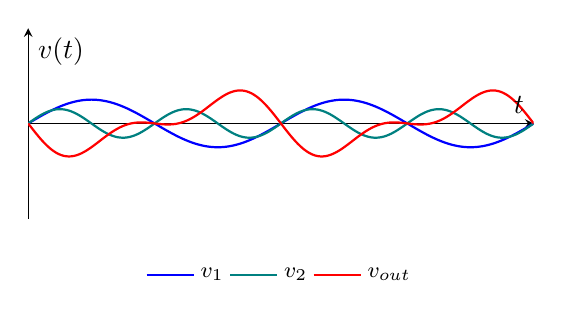
\begin{tikzpicture}
		\begin{axis}[
			width=8cm, height=4cm,
			xlabel={$t$}, ylabel={$v(t)$},
			axis lines=middle,
			ymin=-4, ymax=4,
			xtick=\empty, ytick=\empty,
			domain=0:2, samples=200,
			legend style={draw=none, font=\footnotesize, at={(0.5,-0.2)}, anchor=north, legend columns=3}
			]
			\addplot[blue, thick] {sin(360*x)};
			\addlegendentry{$v_1$}
			\addplot[teal, thick] {0.6*sin(360*2*x)};
			\addlegendentry{$v_2$}
			\addplot[red, thick] {-(sin(360*x) + 0.6*sin(360*2*x))};
			\addlegendentry{$v_{out}$}
		\end{axis}
	\end{tikzpicture}
	\caption{Expected waveforms for the summing amplifier with two sinusoidal inputs of different frequency ($R_1=R_2=R_f$): the output is the inverted sum of the two inputs.}
	\label{fig:wave_adder}
\end{figure}

\begin{figure}[h!]
	\centering
	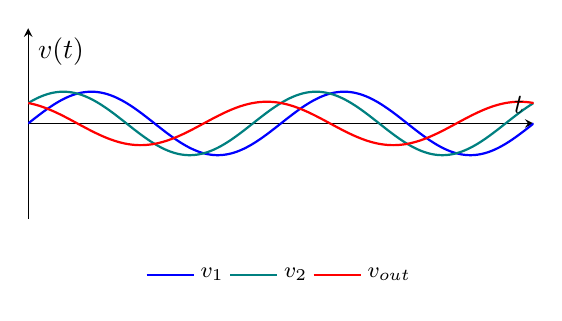
\begin{tikzpicture}
		\begin{axis}[
			width=8cm, height=4cm,
			xlabel={$t$}, ylabel={$v(t)$},
			axis lines=middle,
			ymin=-3, ymax=3,
			xtick=\empty, ytick=\empty,
			domain=0:2, samples=200,
			legend style={draw=none, font=\footnotesize, at={(0.5,-0.2)}, anchor=north, legend columns=3}
			]
			\addplot[blue, thick] {sin(360*x)};
			\addlegendentry{$v_1$}
			\addplot[teal, thick] {sin(360*x+40)};
			\addlegendentry{$v_2$}
			\addplot[red, thick] {sin(360*x+40) - sin(360*x)};
			\addlegendentry{$v_{out}$}
		\end{axis}
	\end{tikzpicture}
	\caption{Expected waveforms for the difference amplifier with two equal-amplitude, equal-frequency inputs of different phase ($R_1=R_2$, $R_f=R_3$): the output amplitude reflects only the phase/amplitude difference between $v_1$ and $v_2$.}
	\label{fig:wave_subtractor}
\end{figure}

\section{Observation Table}

\begin{table}[h!]
	\centering
	\begin{tabular}{@{}cccc@{}}
		\toprule
		$v_1$ (V) & $v_2$ (V) & $v_3$ (V) & $v_{out}$ (V) \\
		\midrule
		&  &  &  \\
		&  &  &  \\
		&  &  &  \\
		&  &  &  \\
		\bottomrule
	\end{tabular}
	\caption{Summing amplifier: DC observation table (measured vs. Equation~\eqref{eq:adder_gain}).}
	\label{tab:adder_obs}
\end{table}

\begin{table}[h!]
	\centering
	\begin{tabular}{@{}ccccc@{}}
		\toprule
		$v_1$ (V) & $v_2$ (V) & $v_{out}$ (theory) & $v_{out}$ (measured) & \% Error \\
		\midrule
		&  &  &  &  \\
		&  &  &  &  \\
		&  &  &  &  \\
		&  &  &  &  \\
		\bottomrule
	\end{tabular}
	\caption{Difference amplifier: DC observation table (including the equal-input common-mode test).}
	\label{tab:subtractor_obs}
\end{table}

\section{Result}

Summing and difference amplifier circuits were designed, assembled using the IC 741, and tested with both DC and AC input signals. The measured output in each case was found to be in close agreement with the theoretical relationships of Equations~\eqref{eq:adder_gain} and~\eqref{eq:subtractor_gain}, and the difference amplifier was verified to substantially reject common-mode input signals when the resistor ratios satisfied Equation~\eqref{eq:cmrr_condition}.

\section{Questions}
\begin{enumerate}[label=Q\arabic*.]
	\item Using the virtual-ground concept, derive Equation~\eqref{eq:adder_gain} for the three-input summing amplifier from first principles.
	\item How would you modify the summing amplifier circuit to perform \emph{subtraction} of two signals using only inverting-adder and inverting-amplifier (unity gain) stages, without using the single-op-amp difference amplifier of Figure~\ref{fig:subtractor}?
	\item Why is the matched-ratio condition of Equation~\eqref{eq:cmrr_condition} important for common-mode rejection in the difference amplifier? What happens to the CMRR if $R_3/R_2 \neq R_f/R_1$?
	\item Define Common-Mode Rejection Ratio (CMRR) and explain why a high CMRR is desirable in instrumentation applications.
	\item What is a key limitation of the single-op-amp difference amplifier of Figure~\ref{fig:subtractor} regarding input impedance, particularly when $R_1$ is small? How does an instrumentation amplifier (using three op-amps) overcome this limitation?
	\item If all three inputs of the summing amplifier in Figure~\ref{fig:adder} are driven with the same DC voltage $V$, and $R_1=R_2=R_3=R_f$, what is $v_{out}$? Verify this against your observation table.
	\item Explain, with an example, one practical application each of a summing amplifier and a difference amplifier in analogue signal processing systems.
\end{enumerate}